
\section{Irregular}
\begin{figure}[h]
\centering
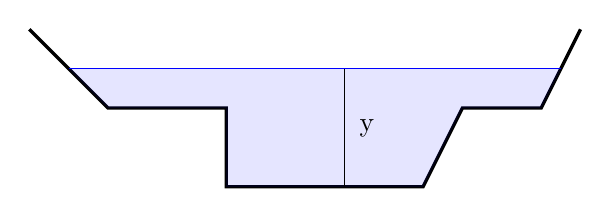
\begin{tikzpicture}
\draw[very thick] (0,0) -- (1,-1) -- (2.5,-1)--(2.5, -2) --(5, -2)-- (5.5, -1) -- (6.5,-1) --(7,0);
\draw[blue] (0.5,-0.5) -- (6.75,-0.5);
\filldraw[fill=blue, opacity=0.1](0.5, -0.5) -- (1,-1) -- (2.5,-1)--(2.5, -2) --(5, -2)-- (5.5, -1) -- (6.5, -1) -- (6.75, -0.5);
\draw (4,-2)--node[right=2]{y} (4,-0.5);
\end{tikzpicture}
\caption{Irregular Section}
\end{figure}

\subsection{Composite Roughness}

\noindent Pavlovskii's method

\noindent Assumption: the total force-resisting motion is equal to the sum of the subsection-resisting forces.

\begin{equation}
nP^2 = \sum n_iP_i^2
\end{equation}

\noindent Horton's method

\noindent Assumption: each subdivision has the same average velocity of the total section
\begin{equation}
Pn^{3/2} = \sum P_i  n_i^{3/2}
\end{equation}

\noindent Colebatch method

\begin{equation}
An^{3/2} = \sum A_i  n_i^{3/2}
\end{equation}

\noindent Cox method

\begin{equation}
An = \sum A_i  n_i
\end{equation}

\noindent Lotter method

\noindent Assumption: the total discharge is eqal to the sum of the subsection discharges.

\begin{equation}
\frac{PR^{5/3}}{n} = \sum \frac{P_i  R_i^{5/3}}{n_i}
\end{equation}
